\section{Experiments and Results}
\label{sec:experiments}

\subsection{Computational and Accuracy Trade-offs}
We evaluate matched decoder pairs across three 3D medical image segmentation backbones: a large-kernel CNN (3D UX-Net \cite{lee20233d}), a vision transformer (SwinUNETR \cite{hatamizadeh2022swin}), and a ConvNeXt-style network (MedNeXt-M-K3 \cite{roy2023mednext}). Benchmarks are conducted across three diverse clinical datasets: the BTCV multi-organ CT dataset (13 organs) \cite{landman2015btcv}, the Medical Segmentation Decathlon Task01 BrainTumour MRI dataset (4-channel brain glioma) \cite{simpson2019large}, and the Medical Segmentation Decathlon Task08 HepaticVessel CT dataset (vessels and tumors) \cite{simpson2019large}.

\textbf{Baseline Comparison}: Table \ref{tab:main_results} summarizes the aggregate computational complexity and segmentation performance under standard end-to-end model training. For each backbone, we evaluate the standard Full decoder ($E_0$) against an Efficient baseline ($E_1$) implementing the parameter reduction strategy of EffiDec3D \cite{effidec3d}. Across all three backbones, $E_1$ achieves substantial FLOP reductions (up to 91.4\% in 3D UX-Net) while retaining competitive Mean Dice scores (e.g., MedNeXt-M-K3 $E_0$ achieves 83.74\% Mean Dice vs. 81.47\% for $E_1$, while $E_1$ reduces inference latency from 40.9 ms to 18.7 ms).

\begin{table*}[tb]
\centering
\caption{Quantitative comparison of Full ($E_0$) vs. Efficient ($E_1$) decoders on the BTCV 13-organ dataset across three backbones.}
\label{tab:main_results}
\small
\begin{tabular*}{\textwidth}{@{\extracolsep{\fill}}lcccccc}
\toprule
\textbf{Architecture} & \textbf{Variant} & \textbf{Params (M)} $\downarrow$ & \textbf{FLOPs (GMac)} $\downarrow$ & \textbf{Latency (ms)} $\downarrow$ & \textbf{Mean Dice (\%)} $\uparrow$ & \textbf{Mean HD95 (mm)} $\downarrow$ \\
\midrule
\multirow{2}{*}{\textbf{3D UX-Net}} & Full ($E_0$) & 53.01 & 578.74 & 40.6 & 79.18 & 9.04 \\
 & Effi ($E_1$) & 3.16 & 49.49 & 8.0 & 77.73 & 11.82 \\
\midrule
\multirow{2}{*}{\textbf{SwinUNETR}} & Full ($E_0$) & 62.19 & 308.24 & 37.0 & 80.48 & 8.88 \\
 & Effi ($E_1$) & 11.21 & 55.84 & 16.7 & 79.49 & 8.90 \\
\midrule
\multirow{2}{*}{\textbf{MedNeXt-M-K3}} & Full ($E_0$) & 39.32 & 230.87 & 40.9 & 83.74 & 5.77 \\
 & Effi ($E_1$) & 12.95 & 106.91 & 18.7 & 81.47 & 6.60 \\
\bottomrule
\end{tabular*}
\end{table*}

\textbf{Factorial Factor Analysis}: In our decoder-isolated attribution analysis on 3D UX-Net with frozen shared encoders (Table \ref{tab:factorial}), we separate channel reduction ($C_{dec}$) from stage removal ($RF$). Reducing channels from 384 to 48 ($C_{48}, RF_1$) compresses parameters from 46.72M to 2.24M while maintaining a 79.80\% Mean Dice. Omitting the high-resolution stage ($C_{384}, RF_2$) reduces latency to 16.1 ms. Combining both ($C_{48}, RF_2$) yields the $E_1$ configuration (1.84M params, 49.49 GMac).

Aggregate metrics confirm the overall efficiency-accuracy trade-off, but they do not reveal where additional decoder computation acts or helps across volumetric space.

\begin{table*}[tb]
\centering
\caption{$2\times2$ Factorial analysis of decoder channel reduction ($C_{dec}$) and resolution scaling ($RF$) on 3D UX-Net (BTCV dataset).}
\label{tab:factorial}
\small
\begin{tabular*}{\textwidth}{@{\extracolsep{\fill}}lcccccc}
\toprule
\textbf{Configuration} & $C_{dec}$ & $RF$ & \textbf{Params (M)} & \textbf{FLOPs (GMac)} & \textbf{Latency (ms)} & \textbf{Mean Dice (\%)} \\
\midrule
Full ($C_{384}, RF_1$) & 384 & 1 & 46.72 & 657.76 & 43.3 & 80.44 \\
Chan-Only ($C_{48}, RF_1$) & 48 & 1 & 2.24 & 388.15 & 35.2 & 79.80 \\
Res-Only ($C_{384}, RF_2$) & 384 & 2 & 46.32 & 319.10 & 16.1 & 77.97 \\
Effi ($C_{48}, RF_2$) & 48 & 2 & 1.84 & 49.49 & 8.0 & 78.35 \\
\bottomrule
\end{tabular*}
\end{table*}

\subsection{Spatial Heterogeneity of Decoder Contribution}

\subsubsection{Global Correction-Degradation Balance}
Evaluating voxel-level prediction shifts between matched $E_0$ and $E_1$ decoders reveals that positive corrections $P(v)$ and negative degradations $N(v)$ are comparable in magnitude across backbones and clinical datasets. The subject-mean net gain $R_{net}$ remains small ($<0.1\%$) across all models: $+0.046\%$ (95\% CI: $[-0.020\%, +0.110\%]$) for 3D UX-Net, $-0.001\%$ (95\% CI: $[-0.045\%, +0.040\%]$) for SwinUNETR, and $+0.085\%$ (95\% CI: $[+0.024\%, +0.152\%]$) for MedNeXt-M-K3 (Figure \ref{fig:heterogeneity}, left column). While 3D UX-Net and SwinUNETR exhibit global confidence intervals crossing zero, MedNeXt-M-K3 shows a small, statistically significant positive shift. Overall, positive voxel corrections are largely counterbalanced by negative degradations across global volumes.

\subsubsection{Boundary Localization of Decoder Activity}
Spatial stratification reveals that decoder activity $A(v) = P(v) + N(v)$ is concentrated near anatomical boundaries across datasets. Error rates in boundary regions are $3.93\times$ higher than in organ interiors for 3D UX-Net and $4.67\times$ higher for MedNeXt-M-K3. Figure \ref{fig:heterogeneity} (right column) shows that both positive corrections and negative degradations peak sharply within a 0--1 voxel boundary band, demonstrating that decoder capacity acts primarily at spatial transitions.

\subsubsection{Factorial Attribution of Channel vs. Stage Interventions}
To isolate the specific architectural mechanisms driving boundary localization, we examine the pairwise spatial flip distributions from our frozen shared-encoder factorial ablation on 3D UX-Net:
\begin{itemize}
    \item \textbf{High-Resolution Stage Removal ($RF_1 \rightarrow RF_2$)}: Removing the high-resolution stage accounts for the majority of compute reduction (657.8 GMac $\rightarrow$ 319.1 GMac). Crucially, the net benefit of retaining this high-resolution stage is sharply boundary-concentrated, yielding a net positive correction rate of $+0.033\%$ in the 0--1 voxel boundary band and $+0.031\%$ in the 1--2 voxel band (both $95\%$ CIs excluding zero), decaying to negative net values ($-0.011\%$) in organ interiors ($>4$ voxels). This establishes that high-resolution decoding stages specifically drive boundary refinement.
    \item \textbf{Channel Width Reduction ($C_{384} \rightarrow C_{48}$)}: Reducing decoder channels compresses parameter count by $95\%$ (46.7M $\rightarrow$ 2.2M) while exerting a spatially diffuse and net-neutral effect ($R_{net} = +0.027\%$, 95\% CI: $[-0.027\%, +0.083\%]$). At the 0--1 voxel boundary, channel reduction produces a slight negative net rate ($-0.020\%$), confirming that channel width provides diffuse representation capacity without driving localized boundary resolution.
\end{itemize}

\subsubsection{Anatomical Volatility}
Anatomical structure analysis (Figure \ref{fig:heterogeneity_anatomy}) demonstrates that small, morphologically complex organs exhibit high flip volatility. The left and right adrenal glands show positive correction rates of 16.2\%/16.9\% in 3D UX-Net, 14.4\%/14.8\% in SwinUNETR, and 18.3\%/10.4\% in MedNeXt-M-K3. Conversely, large structures like the liver remain highly stable ($<3\%$ Activity).

Extra decoder computation is largely inactive in smooth organ interiors, but frequently alters predictions near boundaries and difficult structures.

\begin{figure*}[tb]
\centering
\begin{tabular}{cc}

\includegraphics[width=0.42\textwidth]{figures/obs-uxnet-concat/H1_global_flips.png} &

\includegraphics[width=0.42\textwidth]{figures/obs-uxnet-concat/H2_boundary.png} \\
(a) 3D UX-Net Global Flips & (b) 3D UX-Net Boundary Flips \\[4pt]

\includegraphics[width=0.42\textwidth]{figures/obs-swin-concat/H1_global_flips.png} &

\includegraphics[width=0.42\textwidth]{figures/obs-swin-concat/H2_boundary.png} \\
(c) SwinUNETR Global Flips & (d) SwinUNETR Boundary Flips \\[4pt]
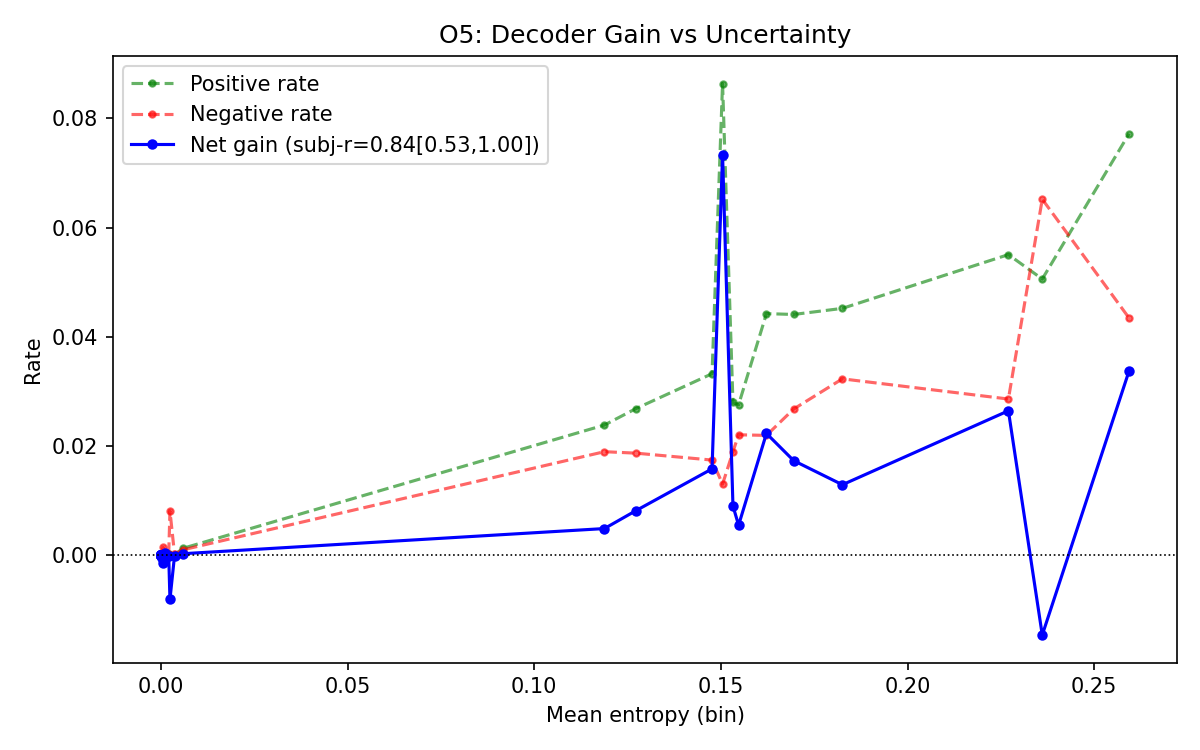
\includegraphics[width=0.42\textwidth]{figures/obs-mednext/O5_decoder_gain.png} &
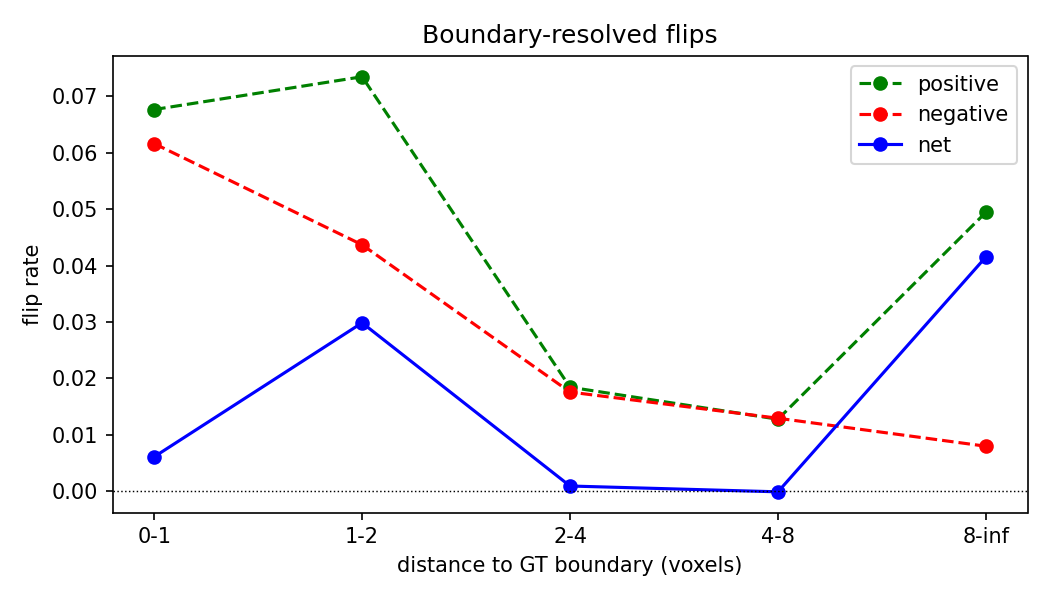
\includegraphics[width=0.42\textwidth]{figures/obs-mednext/O_boundary_flips.png} \\
(e) MedNeXt-M-K3 Global Flips & (f) MedNeXt-M-K3 Boundary Flips \\
\end{tabular}
\caption{Voxel-level net gain and spatial boundary concentration across architectures. Left Column: Global positive corrections, negative degradations, and net gain ($R_{net} < 0.1\%$). Right Column: Activity and net gain as a function of distance to organ boundaries.}
\label{fig:heterogeneity}
\end{figure*}

\begin{figure*}[tb]
\centering

\includegraphics[width=0.85\textwidth]{figures/obs-uxnet-concat/O_anatomy.png} \\
\vspace{-2pt}{\small (a) 3D UX-Net Organ-Level Flips} \\[4pt]

\includegraphics[width=0.85\textwidth]{figures/obs-swin-concat/O_anatomy.png} \\
\vspace{-2pt}{\small (b) SwinUNETR Organ-Level Flips} \\[4pt]
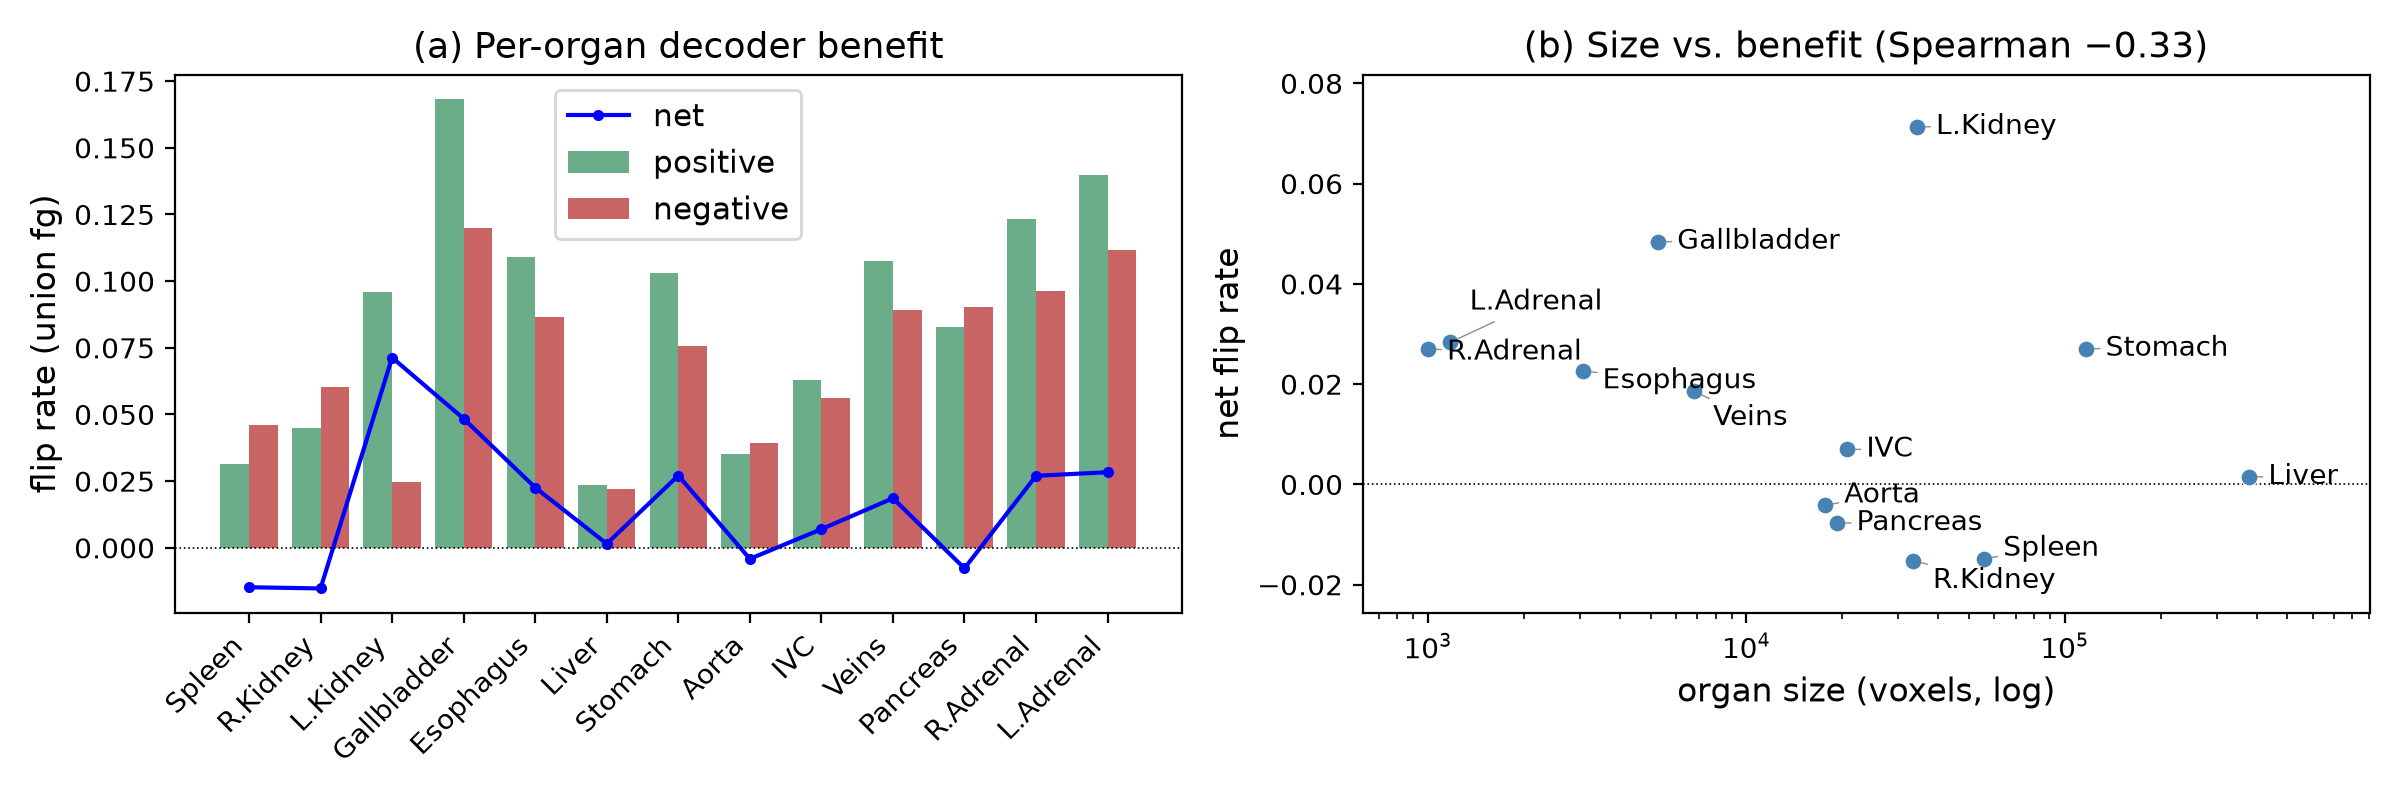
\includegraphics[width=0.85\textwidth]{figures/obs-mednext/O_anatomy.png} \\
\vspace{-2pt}{\small (c) MedNeXt-M-K3 Organ-Level Flips} \\
\caption{Organ-level flip breakdown across backbones. Complex and small anatomical structures show high prediction volatility, whereas large organs remain stable.}
\label{fig:heterogeneity_anatomy}
\end{figure*}

\subsection{Spatial Concentration of Decoder Benefit}
Figure \ref{fig:concentration} presents oracle coverage curves evaluating the spatial concentration of positive net gain $G(r)$. Across all three architectures and datasets, an oracle selecting the top 5\% of blocks recovers 80\% of the full decoder's total positive net gain ($K_{80} = 5\%$). At a 10\% volume budget, oracle coverage reaches 99.98\%, reaching 100\% at 20\%.

The top 5\% of spatial blocks account for 80\% of the observed positive net gain ($K_{80} = 5\%$), indicating strong spatial concentration of beneficial decoder effects. This does not imply that the remaining 95\% of blocks are entirely inactive or dispensable, but rather that high-capacity decoder computation yields diminishing net returns outside this core subset.

\begin{figure}[tb]
\centering

\includegraphics[width=0.82\columnwidth]{figures/obs-uxnet-concat/O_pareto.png} \\
\vspace{-2pt}{\small (a) 3D UX-Net Concentration Curve} \\[4pt]

\includegraphics[width=0.82\columnwidth]{figures/obs-swin-concat/O_pareto.png} \\
\vspace{-2pt}{\small (b) SwinUNETR Concentration Curve} \\[4pt]

\includegraphics[width=0.82\columnwidth]{figures/obs-mednext/O_pareto.png} \\
\vspace{-2pt}{\small (c) MedNeXt-M-K3 Concentration Curve}
\caption{Oracle concentration curves showing that 80\% of positive net gain ($K_{80}$) is concentrated in 5\% of spatial blocks across all three backbones.}
\label{fig:concentration}
\end{figure}

\subsection{Predictability of Decoder Activity and Gain}
We test whether cheap inference-time signals (predictive entropy and TTA mutual information) can locate these beneficial spatial regions prior to full decoder execution. Figure \ref{fig:predictability} and Figure \ref{fig:flip_density} demonstrate a sharp divergence between predicting Activity and predicting Net Gain:
\begin{itemize}
    \item \textbf{Activity Prediction (Flip Location AUROC)}: Predictive entropy reliably identifies active blocks ($A(r) > 0$), achieving high location AUROCs of 0.900 for 3D UX-Net (AUPRC 0.371), 0.913 for SwinUNETR (AUPRC 0.351), and 0.931 for MedNeXt-M-K3.
    \item \textbf{Directional Utility Prediction (Direction AUROC)}: Predictive entropy fails to distinguish positive corrections from negative degradations ($G(r) > 0$ vs. $G(r) < 0$), yielding direction AUROCs near random chance: 0.591 for 3D UX-Net (95\% CI: $[0.558, 0.624]$), 0.560 for SwinUNETR (95\% CI: $[0.514, 0.609]$), and 0.545 for MedNeXt-M-K3. 
    \item \textbf{TTA Mutual Information Diagnostic (TTA-MI)}: Multi-sample epistemic disagreement $I(v)$ over $K=8$ spatial view transformations fails to resolve directional utility, yielding direction AUROCs of 0.539 for 3D UX-Net (95\% CI: $[0.50, 0.58]$) and 0.570 for SwinUNETR (95\% CI: $[0.53, 0.61]$). This confirms that even multi-view epistemic uncertainty cannot predict whether additional decoder capacity yields net improvement.
    \item \textbf{Conditional Density Overlap}: Figure \ref{fig:flip_density} visualizes the conditional entropy density distributions $p(H \mid P(v)=1)$ and $p(H \mid N(v)=1)$. Positive and negative flips exhibit nearly identical high-entropy distributions concentrated at anatomical boundaries, demonstrating why scalar uncertainty signals cannot separate beneficial from harmful decoder interventions.
\end{itemize}

\begin{figure}[tb]
\centering

\includegraphics[width=0.82\columnwidth]{figures/obs-uxnet-concat/O3_entropy_by_flip.png} \\
\vspace{-2pt}{\small (a) 3D UX-Net Flip Entropy Density} \\[4pt]

\includegraphics[width=0.82\columnwidth]{figures/obs-swin-concat/O3_entropy_by_flip.png} \\
\vspace{-2pt}{\small (b) SwinUNETR Flip Entropy Density}
\caption{Conditional entropy density distributions for positive corrections ($P$) and negative degradations ($N$). Overlapping distributions demonstrate why scalar uncertainty signals fail to predict directional net gain.}
\label{fig:flip_density}
\end{figure}

\begin{figure}[tb]
\centering

\includegraphics[width=0.82\columnwidth]{figures/obs-uxnet-concat/O3_unc_error.png} \\
\vspace{-2pt}{\small (a) 3D UX-Net Predictability} \\[4pt]

\includegraphics[width=0.82\columnwidth]{figures/obs-swin-concat/O3_unc_error.png} \\
\vspace{-2pt}{\small (b) SwinUNETR Predictability} \\[4pt]

\includegraphics[width=0.82\columnwidth]{figures/obs-mednext/O3_unc_error.png} \\
\vspace{-2pt}{\small (c) MedNeXt-M-K3 Predictability}
\caption{Inference-time predictability: Predictive entropy reliably identifies active blocks (Location AUROC $>0.90$) but cannot distinguish positive corrections from negative degradations (Direction AUROC $\approx 0.55$).}
\label{fig:predictability}
\end{figure}

\subsection{Macro-Metric Performance Recovery ($R_{\text{recovery}}$)}
Figure \ref{fig:macro_recovery} presents the macro-metric Dice recovery curves $R_{\text{recovery}}(k)$ as a function of the spatial block budget $k\%$. While voxel-level net flips cancel globally ($R_{net} \approx 0$), macroscopic metrics such as Dice and NSD disproportionately reward boundary refinement. 

Routing high-entropy boundary blocks to the full decoder $E_0$ achieves rapid macro-metric recovery:
\begin{itemize}
    \item At a \textbf{5\% block budget}, entropy-guided routing recovers \textbf{60\% of the full decoder's Dice gap} over $E_1$ for 3D UX-Net (compared to 8\% for random selection).
    \item At a \textbf{20\% block budget}, entropy-guided routing achieves \textbf{100\% recovery of the macro Dice gap} across both 3D UX-Net and SwinUNETR (vs. 17--20\% for random selection).
\end{itemize}
This reconciles the apparent paradox between voxel-level net-neutrality and macro-metric improvement: \textit{while additional decoder capacity produces balanced voxel flips overall, the positive flips occur at Dice-sensitive boundary regions, allowing selective boundary decoding to fully recover macro segmentation performance.}

\begin{figure}[tb]
\centering

\includegraphics[width=0.82\columnwidth]{figures/obs-uxnet-concat/R_recovery.png} \\
\vspace{-2pt}{\small (a) 3D UX-Net Macro Dice Recovery} \\[4pt]

\includegraphics[width=0.82\columnwidth]{figures/obs-swin-concat/R_recovery.png} \\
\vspace{-2pt}{\small (b) SwinUNETR Macro Dice Recovery}
\caption{Macro-metric Dice recovery curves ($R_{\text{recovery}}$) showing that entropy-guided selective routing on a 20\% block budget recovers 100\% of the full decoder's macro Dice gap.}
\label{fig:macro_recovery}
\end{figure}
